\chapter{Historie a základní pojmy}
\label{chap:theory}

V této kapitole je ve zkratce popsána historie deskových her, zmíněny některé důležité tituly a představeny základní pojmy herní teorie a designu.


\section{Historický vývoj}
\label{sec:history}

Deskové hry lidstvo provázejí už překvapivě dlouhou dobu. Ať už sloužily jako zábava, nástroj ke vzdělávání nebo jen jako aktivita umožňující sociální kontakt, vždy byly součástí lidské kultury. Vývoj deskových her odráží vývoj lidské civilizace -- změny v technologiích, kultuře a filozofii. Následující sekce přibližují historii, kterou si deskové hry v průběhu času prošly.

\subsection{Počátky}
\label{subsec:beginnings}

Za úplně první deskovou hru by se daly považovat kostky. Ty byly nalezeny v různých prehistorických nalezištích, což znamená, že lidstvo si s nimi hrálo dřív, než začalo zanechávat písemné záznamy. Kromě kostek se však našly i jiné předměty, které byly pravděpodobně používány k hraní her. Šlo například o sadu barevných vyřezávaných kamínků, které byly nalezeny v Turecku, nebo zdobená dřívka z Mezopotámie. \cite{attia_2018}

Nejstarší nalezená desková hra, historiky pojmenovaná \glsref{royal_game_of_ur}, pochází z Mezopotámie. Byla objevena v hrobce krále Ur, který žil před 4500 lety. Hra byla určena pro dva hráče, kteří měli za úkol jako první dopravit své figurky na konec herního pole. Zajímavé také je, že se spolu s hrou uchovala i její pravidla, napsaná v klínovém písmu na destičky. Její věrnou repliku, která je vystavena v Britském muzeu je možné vidět na obrázku \ref{fig:royal_game_of_ur}. Mezi další hry z této doby patří například \glsref{senet}, která byla oblíbená v Egyptě, nebo \glsref{mahjong}, která pochází z Číny. \cite{british_museum_2021}

\begin{figure}[h]
    \centering
    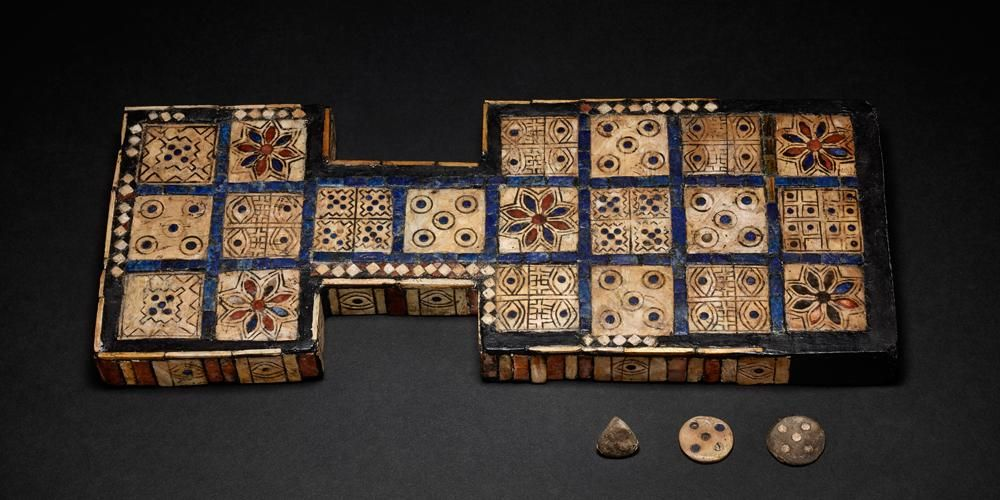
\includegraphics[width=0.7\textwidth]{figures/images/royal-game-of-ur-british-museum.jpg}
    \caption{Replika hry \textit{The Royal Game of Ur} v British Museum. \cite{british_museum_2021}}
    \label{fig:royal_game_of_ur}
\end{figure}

Dále by se do této kategorie daly zařadit i velmi oblíbené \textbf{\glsref{chess}}, které zdánlivě provází lidstvo už od počátků. Jejich historie sahá do roku 400 př. n. l., kdy vznikla keltská hra \glsref{tafl}. Jednalo se o asymetrickou hru, ve které se jeden hráč snažil utéct se svým králem, začínajícím hru ve středu šachovnice, zatímco druhý hráč se snažil krále chytit. Historici se domnívají, že tato verze byla v Indii 6. století našeho letopočtu převzata a pozměněna ve hru \glsref{chaturanga}. Během let její popularita rostla a rozšířila se do celé Asie a nakonec i do Evropy. Do formy, kterou známe dnes, se šachy dostaly právě v Evropě až v 16. století. \cite{chess_com_2023}

Už takhle brzy je tedy možné zaznamenat dodnes využívané herní principy: herní pole složené z políček, po kterých se hráči pohybují podle hodů kostkou, a cíl hry, kterým je dosažení určité pozice na herním poli. \cite{attia_2018}

\subsection{Vývoj deskových her}
\label{subsec:development}

V období od 18. století se deskové hry stávaly více populárnějšími, s čímž se také zvedal zájem o jejich vývoj. Hry byly komplexnější a jejich tvorba se stala výdělečným odvětvím.

Jako jedna z prvních vývojářek deskových her je považována Američanka Elizabeth Magie, která v roce 1903 vytvořila hru \glsref{landlords_game} vyobrazenou na obrázku \ref{fig:landlords-game}. Hra byla zamýšlena jako nástroj k vzdělávání a varování proti rizikům land grabbingu - tedy spekulací s pozemky. Hráči se v ní snažili koupit pozemky, stavět na nich domy a hotely a tím získávat od ostatních hráčů peníze. V roce 1935 Magie prodala patent na hru společnosti Parker Brothers za 500 dolarů. Ti hru přejmenovali na \textbf{\glsref{monopoly}} a začali ji prodávat, což se ukázalo být velmi úspěšné. \cite{attia_2018}

\begin{figure}[h]
    \centering
    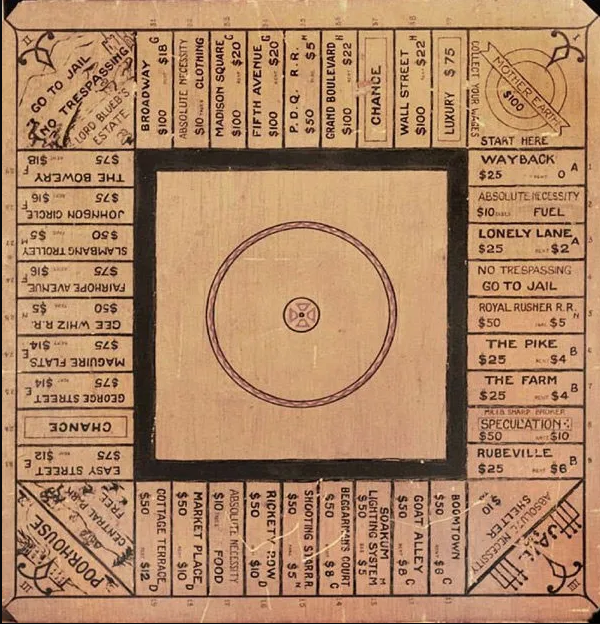
\includegraphics[width=0.3\textwidth]{figures/images/landlords-game.png}
    \caption{Hra \textit{The Landlord's Game} od Elizabeth Magie. \cite{attia_2018}}
    \label{fig:landlords-game}
\end{figure}

V Německu se deskové hry rozrostly tak moc, že se zde okolo nich vytvořila vlastní kultura. V roce 1978 byla založena společnost \textit{Spiel des Jahres}, která každý rok uděluje cenu pro nejlepší hru roku. Tato cena se stala velmi prestižní, zvýšila zájem o deskové hry po celém světě a pomohla k úspěchu mnohým hrám jako \glsref{catan} nebo \glsref{dixit}. \cite{attia_2018}

\subsection{Moderní směr}
\label{subsec:modern}

Kvůli vzniku a úspěchu spousty dalších her, například \glsref{carcassonne}, \glsref{ticket_to_ride} nebo \glsref{risk}, čím dál více lidí chtělo vyvíjet hru vlastní. V tomto jim pomohl jeden z dalších milníků - vznik Kickstarteru. Tato platforma umožňuje vývojářům prezentovat své nápady a získat na ně finanční podporu od lidí, kteří by je chtěli vidět na trhu. \cite{attia_2018}

Díky tomu deskové hry prošly revolucí, neboť nyní zde byla možnost propagovat hru přímo hráčům, kteří by ji chtěli hrát. Velmi úspěšné projekty jako \glsref{exploding_kittens} nebo \glsref{gloomhaven} získaly na Kickstarteru miliony dolarů. Také zde začaly vznikat deskové implementace existujících videoherních titulů, jako například \glsref{darkest_dungeon}, \glsref{witcher} nebo \glsref{dark_souls}. \cite{kickstarter}

Nesmí být opomenut ani gigant mezi deskovými hrami, který přinesl revoluci v herním designu - \textbf{\glsref{dnd}}. Tato hra, vytvořená Gary Gygaxem a Davidem Arnesonem, byla první stolní hrou, která se zaměřovala na příběh a roleplay, neboli hraní určité role v rámci herního světa. Hráči si v ní vytvářeli své postavy a procházeli s nimi dobrodružstvím, které jim připravoval tzv. \textit{Dungeon Master} - hráč, který hru řídil a vytvářel pro ostatní dobrodruhy příběh. Tento nápad byl tak úspěšný, že vytvořil celý žánr - \textit{tabletop RPGs} - a inspiroval spoustu dalších her, jak deskových, tak videoherních. \cite{dnd_beyond_2023}

V moderních hrách je možné pozorovat, že se stále více zaměřují na roleplay a příběh a hlouběji implementují RPG prvky, jako jsou vyvíjející se postavy, dialogy nebo větší důraz na spolupráci mezi hráči. I herní mechanismy se stávají více komplexními a vývojáři se nebojí experimentovat s novými nápady. Hry začínají být i obsáhlejší, což se projevuje v delší době hraní, větší složitosti pravidel a větším množství fyzických komponent.


\section{Definice pojmu desková a stolní hra}
\label{subsec:boardgame_definition}

V této oblasti herního designu se vyskytují dva základní pojmy: \textit{desková hra} a \textit{stolní hra}. Tyto termíny jsou často užívány jako vzájemně zaměnitelné, přestože nesou odlišné významy. V této sekci jsou tyto pojmy podrobněji rozebrány.

\textbf{Desková hra} (board game) je obvykle hra, jejíž hlavní a neoddělitelnou součástí je herní deska. Samotné provedení desky se může lišit, může se jednat o klasickou čtvercovou desku, nebo o jiný tvar, jako například kruhovou, hexagonální nebo jinou. Deska může být také rozdělena na políčka, která mohou mít různé vlastnosti, například barvu, číslo nebo symbol. Hra může mít také další komponenty, jako jsou karty, kostky, figurky, žetony, atd. Herní systém většinou bývá intuitivní a jednoduchý, snažící se zaměřit na širší publikum hráčů. Herní mechaniky se často soustředí na desku a ostatní fyzické komponenty a neobsahují velkou míru abstrakce. Do této kategorie patří například \glsref{monopoly}, \glsref{catan} nebo \glsref{carcassonne}. \cite{board_game_supply_2023}

\textbf{Stolní hra} (tabletop game) je obecnější termín, který zahrnuje všechny hry, které se hrají na stole. To znamená, že do této kategorie můžeme zařadit i hry, které nemají herní desku, jako například karetní hry, hry s kostkami, nebo hry, které se hrají pouze s papírem a tužkou. I když jsou komponenty jejich důležitou součástí, některé stolní hry si dovolují vyšší míru abstrakce herních systémů, což jim dává větší možnosti hloubky na úkor odcizení některých skupin hráčů. Toto můžeme pozorovat například u prosperujícího žánru RPG her, kam můžeme zařadit \glsref{forgotten_waters}, \glsref{gloomhaven} nebo i výše zmíněné \glsref{dnd}. \cite{board_game_supply_2023}

Pro účely této práce bude pozornost věnována především deskovým hrám, přičemž se bude usilovat o zahrnutí některých prvků stolních her, jež by mohly být pro návrh užitečné.
